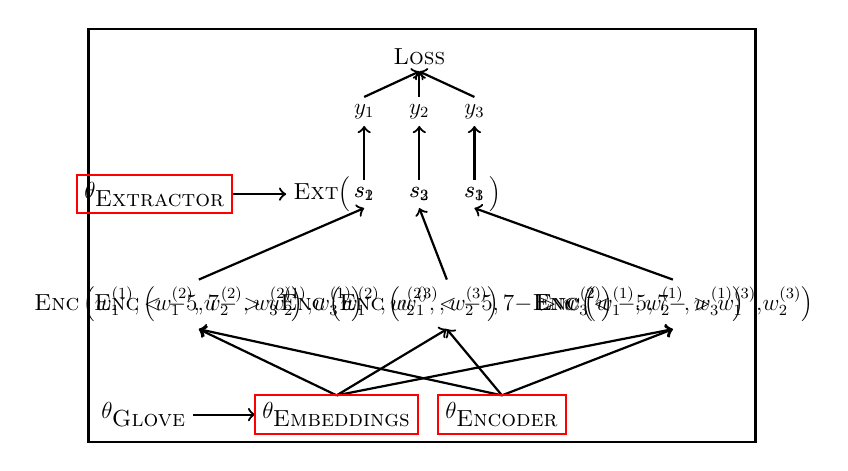
\begin{tikzpicture}[thick,scale=0.7, every node/.style={transform shape}]

  \draw[draw=black] (-2,5) rectangle (10.1,-2.5);

  \uncover<1-6>{
    \node (w1) at (0,0) 
      {\large $\textsc{Enc}\left(w^{(1)}_1,
       \uncover<-5,7->{w^{(1)}_2,} w^{(1)}_3\right)$};
    \node (w3) at (8.6,0) 
      {\large $\textsc{Enc}\left( \uncover<-5,7->{ w^{(3)}_1, }
       w^{(3)}_2 \right)$};
    \node (w2) at (4.5,0) 
      {\large $\textsc{Enc}\left(w^{(2)}_1, 
       w^{(2)}_2,\uncover<-5,7->{  w^{(2)}_3} \right)$};


  }
  
  \uncover<7>{
    \node (w21) at (0,0) 
      {\large $\textsc{Enc}\left(w^{(2)}_1, w^{(2)}_2,w^{(2)}_3 \right)$};
    \node (w13) at (8,0) 
      {\large $\textsc{Enc}\left(w^{(1)}_1, w^{(1)}_2, w^{(1)}_3\right)$};
    \node (w32) at (4,0) 
      {\large $\textsc{Enc}\left(w^{(3)}_1, w^{(3)}_2 \right)$};
  }





  \uncover<1-6>{
    \node (s1) at (3,2) {\large $s_1$};
    \node (s2) at (4,2) {\large $s_2$};
    \node (s3) at (5,2) {\large $s_3$};
  }
  \uncover<7>{
    \node (s13) at (5,2) {\large $s_1$};
    \node (s21) at (3,2) {\large $s_2$};
    \node (s32) at (4,2) {\large $s_3$};
  }


    \draw[->,thick] (w1.north) -- (s1.south); 
    \draw[->,thick] (w2.north) -- (s2.south);
    \draw[->,thick] (w3.north) -- (s3.south);

    \node (ext) at (3.6,2) {\large $\textsc{Ext}\Big( 
        \quad\quad\quad\;\;\;\;\;\;\;\;\;\;\; \Big)$};
\uncover<2->{
    \node (extp) at (-.8,2) {\large $\theta_\textsc{Extractor}$};
    \node (encp) at (5.5,-2) {\large $\theta_\textsc{Encoder}$};
    \draw[->,thick] (encp.north) -- (w1.south);
    \draw[->,thick] (encp.north) -- (w2.south);
    \draw[->,thick] (encp.north) -- (w3.south);
    \draw[->,thick] (extp.east) -- (ext.west);
}

\uncover<3->{
    \node (embp) at (2.5,-2) {\large $\theta_\textsc{Embeddings}$};
    \draw[->,thick] (embp.north) -- (w1.south);
    \draw[->,thick] (embp.north) -- (w2.south);
    \draw[->,thick] (embp.north) -- (w3.south);
}
\uncover<4->{
        \draw[draw=red] (extp.north east) rectangle (extp.south west);
       \draw[draw=red] (encp.north east) rectangle (encp.south west);
    \node (glovep) at (-1,-2) {\large $\theta_\textsc{Glove}$};
    \draw[->,thick] (glovep.east) -- (embp.west);

}
\uncover<5>{
        \draw[draw=red] (embp.north east) rectangle (embp.south west);
}
    \node (y1) at (3,3.5) {\large $y_1$};
    \node (y2) at (4,3.5) {\large $y_2$};
    \node (y3) at (5,3.5) {\large $y_3$};
    \draw[->,thick] (s1.north) -- (y1.south);
    \draw[->,thick] (s2.north) -- (y2.south);
    \draw[->,thick] (s3.north) -- (y3.south);

    \node (loss) at (4, 4.5) {\large \textsc{Loss}};
    \draw[->,thick] (y1.north) -- (loss.south);
    \draw[->,thick] (y2.north) -- (loss.south);
    \draw[->,thick] (y3.north) -- (loss.south);
 

%    \uncover<2->{   
 %      \draw[->,thick,red] (loss.south) + (-5mm, 0) -- (y1.north west);
 %      \draw[->,thick,red] (loss.south) + (5mm, 0) -- (y3.north east);
 %   }
 %   \uncover<3->{
 %      \draw[->,thick,red] (y1.north west) -- (s1.north west);
 %      \draw[->,thick,red] (y3.north east) -- (s3.north east);
 %   }
 %   \uncover<4->{
 %      \draw[->,thick,red] (s1.north west) -- (extp.north east) ;
 %   }
 %   \uncover<5->{
 %      \draw[->,thick,red] (s1.south west)+(-5mm,0) -- (-.7, .6) ;
 %      \draw[->,thick,red] (s3.south east)+(5mm,0) -- (9.2, .6) ;
 %   }
%    \uncover<6->{
 %      \draw[->,thick,red] (-.7, -.5) -- (encp.north west) ;
 %      \draw[->,thick,red] (9.2, -.5) -- (encp.north east) ;
 %      \draw[->,thick,red] (w2.south)+(-2mm,0) -- (4.3, -1.5) ;
  %  }
    

\end{tikzpicture}
